\documentclass[12pt]{article}
\usepackage{fullpage,graphicx,psfrag,amsmath,amsfonts,amsthm,verbatim}
\usepackage[small,bf]{caption}
\usepackage{graphicx}
\usepackage{probsoln}
\usepackage{enumitem}
\usepackage{import}
\usepackage{xifthen}
\usepackage{pdfpages}
\usepackage{transparent}

\newcommand{\ones}{\mathbf 1}
\newcommand{\reals}{{\mbox{\bf R}}}
\newcommand{\integers}{{\mbox{\bf Z}}}
\newcommand{\symm}{{\mbox{\bf S}}}  % symmetric matrices

\newcommand{\nullspace}{{\mathcal N}}
\newcommand{\range}{{\mathcal R}}
\newcommand{\Rank}{\mathop{\bf Rank}}
\newcommand{\Tr}{\mathop{\bf Tr}}
\newcommand{\diag}{\mathop{\bf diag}}
\newcommand{\card}{\mathop{\bf card}}
\newcommand{\rank}{\mathop{\bf rank}}
\newcommand{\conv}{\mathop{\bf conv}}
\newcommand{\prox}{\mathbf{prox}}

\newcommand{\Expect}{\mathop{\bf E{}}}
\newcommand{\Prob}{\mathop{\bf Prob}}
\newcommand{\Co}{{\mathop {\bf Co}}} % convex hull
\newcommand{\dist}{\mathop{\bf dist{}}}
\newcommand{\argmin}{\mathop{\rm argmin}}
\newcommand{\argmax}{\mathop{\rm argmax}}
\newcommand{\epi}{\mathop{\bf epi}} % epigraph
\newcommand{\Vol}{\mathop{\bf vol}}
\newcommand{\dom}{\mathop{\bf dom}} % domain
\newcommand{\intr}{\mathop{\bf int}}
\newcommand{\sign}{\mathop{\bf sign}}

\newcommand{\cf}{{\it cf.}}
\newcommand{\eg}{{\it e.g.}}
\newcommand{\ie}{{\it i.e.}}
\newcommand{\etc}{{\it etc.}}


\title{HW1: Convex sets}
\author{Matrix}

\begin{document}
\maketitle

Homework 1, due Friday 7/1/22:  2.9, 2.12a-e, 2.15, 2.4, A1.4, A2.7, 2.13.

\begin{solution}[2.9(a)]

	\textit{Voronoi region} definition yields
    \begin{align*}
			\|x-x_0\|_2\le \|x-x_i\|_2 & \Longleftrightarrow (x-x_0)^T(x-x_0) \le (x-x_i)^T(x-x_i) \\
															 &\Longleftrightarrow x^Tx-2x_0^Tx+x_0^Tx_0\le x^Tx-2x_{i}^Tx+x_{i}^Tx_{i}\\
															 &\Longleftrightarrow (x_i-x_0)^Tx \le \frac{1}{2}(x_i-x_0)^T(x_i+x_0)
    .\end{align*}
		
		The result above defines a halfspace for each $i$. Thus, we can express  $V$ in the form  $V=\{ x \mid Ax \preceq b\}$ with
		\begin{align*}
			A = \begin{bmatrix} (x_{1}-x_0)^T \\ \vdots \\ (x_{K}-x_0)^T \end{bmatrix} ,\ b=\begin{bmatrix} \frac{1}{2}(x_1-x_0)^T(x_1+x_0) \\ \vdots \\ \frac{1}{2}(x_K-x_0)^T(x_K-x_0) \end{bmatrix} 
		.\end{align*}

\end{solution}

\begin{solution}[2.9(b)]

	Since polyhedron $P$ has nonempty interior, we can express $P$ in the form $P=\{ x \mid Ax \preceq b\}$\footnote{If $P$ only contains hyperplane, then $P$ has empty interior, contradicting the assumption. This form contains both hyperplanes and halfspaces.} with $A \in \reals^{K\times n} $ and $b\in \reals^{K} $.
	We can choose any point $x_0$ from $P$'s interior, then take a mirror image of $x_0$ with respect to a hyperplane $\{a_i^T x = b_i\}$ with $a_{i} = (x_{i}-x_0)$ and $b_{i} = \frac{1}{2}(x_i-x_0)^T(x_i-x_0)$ to get $x_{i}$.
	Thus, any point $x\in P$ has shorter (or equal, when on hyperplane) distance to $x_0$ than $x_{i}$.

	The mirror image $x_{i}$ of $x_0$ with respect to hyperplane $\{a_i^T x = b_i\}$ satisfies
	\begin{align*}
		\begin{cases}
		\frac{\|a_{i}^{T} x_0-b_{i}\|}{\|a_{i}\|} =	\frac{\|a_{i}^{T} x_i-b_{i}\|}{\|a_{i}\|} \Longleftrightarrow a_{i}^{T} x_0-b_{i} = -1\cdot(a_{i}^{T} x_i-b_{i}), \\
x_{i} = x_0 + \lambda a_{i}.
		\end{cases}
	\end{align*}

	Solving $\lambda$ yields:
	\begin{align*}
		\lambda = \frac{2(b_{i}-a_{i}^Tx_0)}{\|a_{i}\|^2}
	.\end{align*}
	Thus, we can choose  
	\begin{align*}
		x_{i} = x_0 + \frac{2(b_{i}-a_{i}^Tx_0)}{\|a_{i}\|^2}a_{i},\ i = 1, \ldots, K
	\end{align*}
	so that the polyhedron $P$ is the \textit{Voronoi region} of $x_0$ with respect to $x_1,\ldots, x_{K}$.

\end{solution}

\begin{solution}[2.9(c)]

	A polyhedron decomposition of $\reals^n$ can not always be described as the \textit{Voronoi regions}.

	There is a counterexample in $\reals^2$ plane, shown in figure \ref{fig:-figures-hw1-29-png}.
	Consider a polyhedron decomposition with respect to two hyperplanes $H_1$ and $H_2$, which yields four polyhedrons $P_1$, $P_2$, $P_3$ and $P_4$.
	Suppose $P_1$ is a \textit{Voronoi region}, then choose any of point $x_1\in P_1$, its mirror image $x_3$ with respect to $H_2$ must be in $\tilde{P}_1\subset P_3$.
	Now we consider $P_2$ as another \textit{Voronoi region}, its mirror image $x_3$ with respect to $H_1$ must be in $\tilde{P}_2\subset P_3$. There is not such point $x_3\in P_3$ satisfying the two conditions.
	\begin{figure}[htpb]
		\centering
		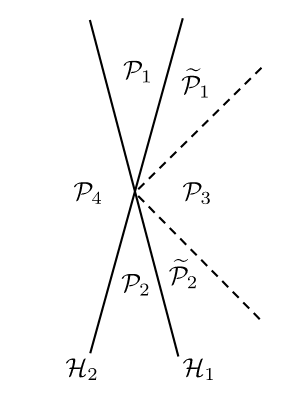
\includegraphics[width=0.2\textwidth]{../figures/hw1-29.png}
		\caption{Polyhedral decomposition/Voronoi region partition counterexample in $\reals^2$}
		\label{fig:-figures-hw1-29-png}
	\end{figure}
	
\end{solution}

\begin{solution}[2.12(a)-(e)]
	\begin{enumerate}[label=(\alph*)]
		\item \textit{salb}: $\left\{ x\in\reals^n \mid \alpha \le a^Tx\le \beta \right\} $.
			Choose any two point $x_1$ and $x_2$ in \textit{slab}.
			For any $\theta\in \left[ 0, 1 \right] $ we have convex combination
			\begin{align*}
				\alpha \le \theta a^Tx_1+(1-\theta)a^Tx_2\le \beta
			.\end{align*}
			Thus, \textit{slab} is convex set.
		\item \textit{rectangle}: $\left\{ x\in \reals^n \mid \alpha_i\le x_{i}\le \beta_{i},\ i=1,\ldots,n\right\} $.
			For any two point $x$ and $y$ in \textit{rectangle} and $\theta \in \left[ 0, 1 \right] $, we have convex combination
			\begin{align*}
				\alpha_i\le \theta x_{i}+(1-\theta)y_{i} \le \beta_{i},\ i=1,\ldots,n
			.\end{align*}
			Thus, \textit{rectangle} is convex set.
		\item \textit{wedge}: $\{x\in{\reals}^{n}\mid a_{1}^{T}x\leq b_{1},\ a_{2}^{T}x\leq b_{2}\}.$
			For any two point $x$ and $y$ in \textit{wedge} and $\theta \in \left[ 0, 1 \right] $, we have convex combination
			\begin{align*}
				\theta a_1^Tx + (1-\theta)a_1^Ty\le b_1,\ \theta a_2^Tx + (1-\theta)a_2^Ty\le b_2
			.\end{align*}
			Thus, \textit{wedge} is convex set.
		\item Set: $\left\{ x \mid \|x-x_0\|_2 \le \|x-y\|_2 \text{ for all } y\in S \right\} $ where $S\subseteq \reals^n$. From the definiton, we have the following:
			\begin{align*}
			\|x-x_0\|_2\le \|x-y\|_2 & \Longleftrightarrow (x-x_0)^T(x-x_0) \le (x-y)^T(x-y) \\
															 &\Longleftrightarrow x^Tx-2x_0^Tx+x_0^Tx_0\le x^Tx-2y^Tx+y^Ty\\
															 &\Longleftrightarrow (y-x_0)^Tx \le \frac{1}{2}(y-x_0)^T(y+x_0)
			.\end{align*}
			Choose any two point $x_1$ and $x_2$ in set.
			For any $\theta\in \left[ 0, 1 \right] $ we have convex combination
			\begin{align*}
				\theta(y-x_0)^Tx_1 + (1-\theta)(y-x_0)^Tx_2 &\le \theta \cdot \frac{1}{2}(y-x_0)^T(y+x_0)\\ &+ (1-\theta) \cdot \frac{1}{2}(y-x_0)^T(y+x_0) \\&= \frac{1}{2}(y-x_0)^T(y+x_0)
			.\end{align*}
			Thus, the set is convex.
		\item Set: $\left\{ x \mid \dist(x,S)\le \dist(x,T) \right\} $ where $S,T\subseteq \reals^n$, and  $\dist(x,S)=\inf \left\{ \|x-z\|_2  \mid z\in S\right\} $. 
			For any norm, we have the following for any two points $x_1$ and $x_2$ in $\reals^n$ and $\theta\in\left[ 0,1 \right] $:
			\begin{align*}
				\|\theta x_1+(1-\theta)x_2-z\|_2 &= \|\theta(x_1-z)+(1-\theta)(x_2-z)\|_2\\
																				 &\le \theta \|x_1-z\|_2 + (1-\theta) \|x_2-z\|_2,\ \forall z\in \reals^n
			.\end{align*}
			Consider $x_1$ and $x_2$ in the set, we have convex combination
			\begin{align*}
				\dist(\theta x_1+(1-\theta)x_2, S) &\le \theta \dist(x_1, S) + (1-\theta)\dist(x_2, S) \\
																					 &\le \theta \dist(x_1, T) + (1-\theta)\dist(x_2, T)
			.\end{align*}
			We can not conclude that $\dist(\theta x_1+(1-\theta)x_2, S) \le \dist(\theta x_1+(1-\theta)x_2, T)$ from above results.

			\textbf{The set is not convex}, with a counterexample in $\reals^2$ shown in figure \ref{fig:-figures-hw1-212e-pdf}. With $S$ (dark area) and $T$ (green area) both are non-convex set, the set (pink area) is not convex\footnote{This is not a rigious proof. Suppose $S=\left\{ -1, 1 \right\}$ and $T=\left\{ 0 \right\} $, the set $\left\{ x| x\le -0.5, x\ge 0.5 \right\} $ is non-convex}.
			\begin{figure}[htpb]
				\centering
				\def\svgwidth{.6\columnwidth}
			\import{../figures/}{hw1-212e.pdf_tex}
				\caption{2.12(e) counterexample with non-convex set in $\reals^2$}
				\label{fig:-figures-hw1-212e-pdf}
			\end{figure}
	\end{enumerate}
	
\end{solution}

\begin{solution}[2.15]
	
\end{solution}

\begin{solution}[2.4]

	\begin{align*}
		\conv\left\{ v_1,\ldots,v_k \right\} =\{\theta_{1}v_{1}+\cdots+\theta_{k}v_{k}\mid \theta \preceq 0,\ \ones^T\theta=1\}
	.\end{align*}
	
\end{solution}

\begin{solution}[A1.4]
	
\end{solution}

\begin{solution}[A2.7]
	
\end{solution}

\begin{solution}[2.13]
	
\end{solution}

\end{document}
